\documentclass{article}

\usepackage{newcent}
\usepackage{algorithm, algorithmic, amsmath, amssymb, amsthm,graphicx}
\usepackage{lscape}
\usepackage{rotating}% provides a rotate environment
\newcommand{\rotxc}[1]{\begin{sideways}#1\end{sideways}}
\newcommand{\invert}[1]{\rotxc{\rotxc{#1}}}

\newcommand{\prom}[1]{\Rsh_{\tt#1}}
\newcommand{\term}{\intercal}
\newcommand{\rrecsite}[1]{\triangleright_{\tt#1}}
\newcommand{\lrecsite}[1]{\triangleleft_{\tt#1}}
\newcommand{\gene}[1]{\framebox{\tt #1}}

\newtheorem{mydef}{Definition}

\textheight 9in
\textwidth 6.5in
\oddsidemargin 0in
\evensidemargin 0in
\headsep 0in
\topmargin -0.5in

\title{Notes on a Bio-automaton}

\author{
Tao / Bhatia
}

\date{}

\begin{document}

\maketitle
\thispagestyle{empty}

\section{Introduction}

We propose an algorithm for generating a plasmid design that implements a given deterministic acyclic
finite automaton using cellular transcriptional machinery. We propose a composable primitive, which
we call the $\tau$-module, to implement our design.


\begin{mydef}
A $\tau$-module$(\alpha,i,j,S)$ is a segment of DNA comprising the following parts in the following order:
\begin{enumerate}
\item A strong bidirectional terminator;
\item A promoter induced by $\alpha$ flanked by co-oriented recombinase $i$ recognition sites;
\item A strong bidirectional terminator flanked by co-oriented recombinase $j$ recognition sites, where $i\neq
j$;
\item A set $S$ of sequences coding for recombinases; and 
\item A strong bidirectional terminator.
\end{enumerate}
\end{mydef}


\begin{mydef}
A deterministic acyclic finite automaton is a tuple $\mathcal{A} = (Q, \Sigma, \delta, s, F)$, where
$Q$ is a finite nonempty set of states, $\Sigma$ is a finite nonempty set of symbols, $\delta: Q
\times \Sigma \rightarrow Q$ is a transition function, $s$ is the initial state, and $F$ is the set
of final states.
\end{mydef}

For our bio-automaton, we interpret $\Sigma$ to be a set of inducers and $F$ to be the set of states
in which a reporter is produced.  The various states of this bio-automaton can be visually represented with an acyclic graph in which states are represented by vertices and inducers are represented by arcs connecting two vertices.  A bio-automaton described by Definition 2 can be constructed out of $n$ $\tau$-modules  where $n$ corresponds to the number of of arcs in the graphs.  With two exceptions, a bio-automaton can be constructed out of $n$ $ \tau$-modules.  

\begin{enumerate}
\item Promoters 'active' in the initial state of the promoter should not be followed by a strong bidirectional terminator flanked by co-oriented matching recombinase recognition sites.  The term active describes a promoter that will allow for the translation of a meaningful product before encountering a terminator. 
\item A $\tau$-module corresponding to a final state need not contain recombinase coding regions.  Recombinase coding regions may be substituted with reporter gene coding regions.  A final state refers to any state that corresponds to the last vertice encountered in a depth first traversal of the graph corresponding the bio-automaton described here.	
\end{enumerate}

\begin{algorithm}
\caption{\sc Bio-automaton generator}
\begin{algorithmic}[1]
    \REQUIRE Deterministic acyclic finite automaton $\mathcal{A} = (Q, \Sigma, \delta, s, F)$
    \STATE $r \leftarrow 0$, $i \leftarrow 0$
    \STATE $A \leftarrow \epsilon$
    \FOR{each state $s$ in $Q$}
        \FOR{each arc $e_i = (s, y, \alpha)$}
            \STATE $p_i \leftarrow r$, $t_i \leftarrow r+1$
            \STATE $C_i \leftarrow C_i \cup p_i$
            \STATE $r \leftarrow r+2$
            \STATE $T_i \leftarrow \tau\textrm{\it-module}(\alpha, p_i, t_i, C_i)$
        \ENDFOR
        \FOR{each arc $e_i=(s, y, \alpha)$}
            \FOR{each arc $e_j=(s, w, \alpha) \neq e_i$}
                \STATE $C_i = C_i \cup \{j\}$
            \ENDFOR
        \ENDFOR
        \FOR{each pair of arcs $e_i=(x, s, \alpha)$ and $e_j = (s, y, \beta)$}
            \STATE $C_i \leftarrow C_i \cup \{t_j\}$
        \ENDFOR
    \ENDFOR
    \STATE Output $T_1 \cdot T_2 \cdot \cdots \cdot T_{|\delta|}$
\end{algorithmic}
\end{algorithm}
\newpage%might have to remove this later...
\section{A Proof of Concept}
The translation of abstract computer science to physical constructs composed of nucleic acids is an exciting capability that may allow synthetic biologists to leverage the extensive work of computer scientists.  However, the bio-automatons proposed here remain abstract and no more than a fanciful dream unless sufficiently grounded by a proof of concept construct.  Such a proof of concept is described below using symbology given in Table 1.\\
 \\
$\term \rrecsite{0} \prom{0} \rrecsite{0} \gene{0} \term\\ 
\term \rrecsite{0} \prom{1} \rrecsite{0} \gene{RFP} \term\\
\term \rrecsite{1} \prom{2} \rrecsite{1} \rrecsite{0} \term \rrecsite{0} \gene{1} \gene{2} \term\\
\term \prom{3} \rrecsite{2} \term \rrecsite{2} \gene{GFP} \term$\\
 \\
The numbers in this design can be substituted for actual recombinase and promoters of course.  All producers in the design is an inducible promoter.  Given that inducible promoters are better characterized than recombinase and that there is a large variety of promoters, specific promoter names will not be provided below.  The following design replaces the numerical subscripts for recombinase recognition sites and recombinase coding regions with the actual recombinase.  The recombinases used in the design are Cre, Dre, and FlpSc.  Each of these recombinase will recognize a pair of recognition sites, and then excise the content in between the sites; one recognition site is removed in the process. Dre and FlpSc can recognize one pair of sites each; Cre and recognize as many as three.
\\
 \\
$\term \rrecsite{Cre} \prom{0} \rrecsite{Cre} \gene{Cre} \term\\ 
\term \rrecsite{Cre} \prom{1} \rrecsite{Cre} \gene{RFP} \term\\
\term \rrecsite{Dre} \prom{2} \rrecsite{Dre} \rrecsite{Cre} \term \rrecsite{Cre} \gene{Dre} \gene{FlpSc} \term\\
\term \prom{3} \rrecsite{FlpSc} \term \rrecsite{FlpSc} \gene{GFP} \term$\\
\newpage%remove this later
\begin{center}
\begin{table}
\centering
\begin{tabular}{| c | l|} 
\hline
Symbol & Meaning\\
\hline
$\prom{0}$ & Promoter\\
$\term$ & Terminator\\
$\lrecsite{0}$, $ \rrecsite{0}$ & Recombinase recognition site\\
$\gene{0}$ & Recombinase coding region\\
$\gene{GFP}$ & Gene coding region\\
\hline
\end{tabular}
\caption{Table 1- Bio-automaton design symbology}
\end{table}
\end{center}
\begin{figure} [h!]
\centering
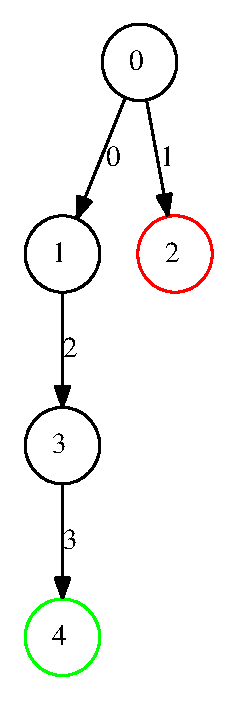
\includegraphics{tree2.eps}
\caption{The bioautomaton described by the proof of concept construct is described by the following graph. States are represented by vertices and each arc corresponds to an inducible promoter}
\end{figure}

\newpage%remove this later
The construct will demonstrate the following:
\begin{enumerate}
\item The design pattern, whereby a state machine is refactored as a set of $\tau$-modules, is feasible, and has behavior that corresponds to the automaton described in Definition 1.
\item The design pattern is potentially scalable given sufficient components such as recombinase and inducible promoters.
\item The $\tau$-module offers clear advantages over the Single Invertase Memory Module created by Collins et al.  These advantages are detailed in the advantages section.
\item The various states of the bio-automaton can be distinguished from one another by observing responses from various reporter genes.
\end{enumerate}
\section{Positive Points}
\begin{enumerate}
\item Arrangement of modules is trivial.  Any permutation of the constituent modules of a design will give a bio-automaton with behavior equivalent to any other permutation; this may be leveraged to produce constructs that reside on multiple plasmids.
\item Provides a clear way to produce excusive arcs.  Suppose that several arcs branch out from a node in the state machine graph.  An exclusive arc should render it impossible to traverse the other arcs from the given node. 
\item Allows for the repeat use of promoters while still allowing for distinct final words; a final word is a set of inputs that result in a reporter response
\item Easily allows for branching designs
\item Supposing only full words need to be recognized, intermediate states may share recombinase, allowing for didesigns that use fewer types of recombinase 
\end{enumerate}

Assuming that constructs built using paradigms outlined here possess physical behavior akin to the behavior asserted here, then $\tau$-module can be a boon to synthetic biology. Our software posesses capability to translate a directed graph to a bio-automaton design.  Each arc is translated individually without information beyond which arcs intersect with a given arc. The minimal use of contextual information during each arc translation indicates that each operation is essentially, independent.  Use of the $\tau$-module offers composability. Composability is a valuable characteristic to automated work flows. If the software that generates the bio-automaton can perform independent optimization operations on each module, then the software can deliver scalable, complex designs, which are difficult to generate by hand. Such tools and design architectures will be common in the next generation of synthetic biological work.  No longer will sofware merely mimic human chores, but software tools will enhance and further human aims and efforts.   
\section{Optimization}
The composable nature of designs using the $\tau$-module described here offers the opportunity to perform optimizations on a design on an arc to arc basis; each arc corresponds to one $\tau$-module.  Such an optimization would examine each module iteratively and perform the appropriate optimizations.  The only necessary contextual would be the module itself, and its immediate neighbors.  Such an optimization method would scale easily with any design, regardless of the complexity.\\

The first of these optimizations involve a merging of modules that represent a set of forwardly-oriented arcs diverging from one common vertex.  Each $\tau$-module diverging from this node uses one recombinase to excise its own promoter to prevent excessive translation of recombinase; another recombinase is used to remove the promoter of each $\tau$-module that diverge from the aforementioned common vertex.  The use of a recombinase in one $\tau$-module removing a promoter in another $\tau$-module allows for the exclusive paths when traversing the graph corresponding to our bioautomaton.  Such a use of recombinase is nontrivial, and can become expensive in terms of recombinase use in a bioautomaton with widely branching states. Examine the following graph, which contains just one fork.
\\
\begin{figure} [h!]
\centering
\includegraphics{tree.eps}
\caption{A graph describing an automaton that has two states that fork from the initial state}
\end{figure}
\\
The unoptimized construct given by the algorithm described in the introduction is as follows: 
\\
%unoptimized construct
$\term \rrecsite{0} \rrecsite{4} \prom{0} \rrecsite{4} \rrecsite{0} \gene{0} \gene{1} \gene{2} \term \\
\term \rrecsite{1} \rrecsite{3} \prom{1} \rrecsite{3} \rrecsite{1} \gene{3} \gene{4} \gene{5} \term \\
\term \prom{2} \rrecsite{2} \term \rrecsite{2} \gene{R0} \term\\
\term \prom{3} \rrecsite{5} \term \rrecsite{5} \gene{R1} \term$\\
\\
The design uses a total of 6 different recombinase, assuming that recombinases use can recognize only one set of recognition sites.
\\
The simple, unoptimized designs can be improved upon by 'merging' several $\tau$-modules together.  Each of the merged modules must diverge from the same vertice and share the same orientation; we will cause these modules 'neighbors'.  Each of these modules contains a recombinase that removes the modules own promoter, and another recombinase that excises the promoter of $\tau$-modules that also diverge from the same state.  In the particular case of several arcs that diverge from the same vertice,  the two recombinase described, are redundant.  By enclosing a module and each of its neighbors in the recognition sites that would be used to cut out the module's own promoter, no additional recombinase need to be used to excise the promoter's of neighbors.  Instead neighboring modules are excised in their entirety, producing the excusive paths described previously.  The reduced use of recombinase should scale exponentially with the number of $\tau$ modules with neighbors, and the number of neighbors each of these modules has.  One recombinase for each neighbor is used in the unoptimized design to remove the promoters of neighbors.  And so supposing there are $n$ modules with neighbors.... ADD MATH TO DESCRIBE HOW MUCH IS SAVED
\\  
%optimized construct
$\rrecsite{0} \rrecsite{3} \prom{1} \rrecsite{3} \rrecsite{5} \term \prom{0} \rrecsite{0} \rrecsite{2} \term \rrecsite{3} \rrecsite{0}\\
\term \prom{2} \rrecsite{2} \term \rrecsite{2} \gene{R0} \term \\
\term \prom{3} \rrecsite{5} \term \rrecsite{5} \gene{R1} \term $\\
\\
\section{Future Work}
Here are a few items to pursue in the future:
\begin{enumerate}
\item Construction and characterization of a physical sample
\item Generation of permutations of parts. 
\item Control module for two cells that talk to each other.
\item DNA security and authentication
\item NOR gates and other logic gates
\end{enumerate}
\end{document}
